\documentclass[../../main.tex]{subfiles}

\begin{document}

\section{Introduction}

Convolutional Neural Networks (CNNs) have been the state of the art in many image processing tasks \parencite{he2015deep, simonyan2015deep, NIPS2012_c399862d}, due to their ability to learn spatial patterns in the data via convolutional filters. Since convolutions are translation equivariant, CNNs learns to recognize patterns regardless of their position in the image, making them desirable for a wide range of tasks, such as image classification, object detection, and segmentation. The performance of CNNs has made them to be a desirable backbone for a Neural Process, motivating the development of the Convolutional Neural Processes (ConvNPs) \parencite{gordon2020convolutional}. We will briefly discuss the ConvNP model and its architecture however for a more comprehensive  explanation, we refer the reader to the original paper.

\section{Architecture}

\begin{figure}[H]
	\centering
	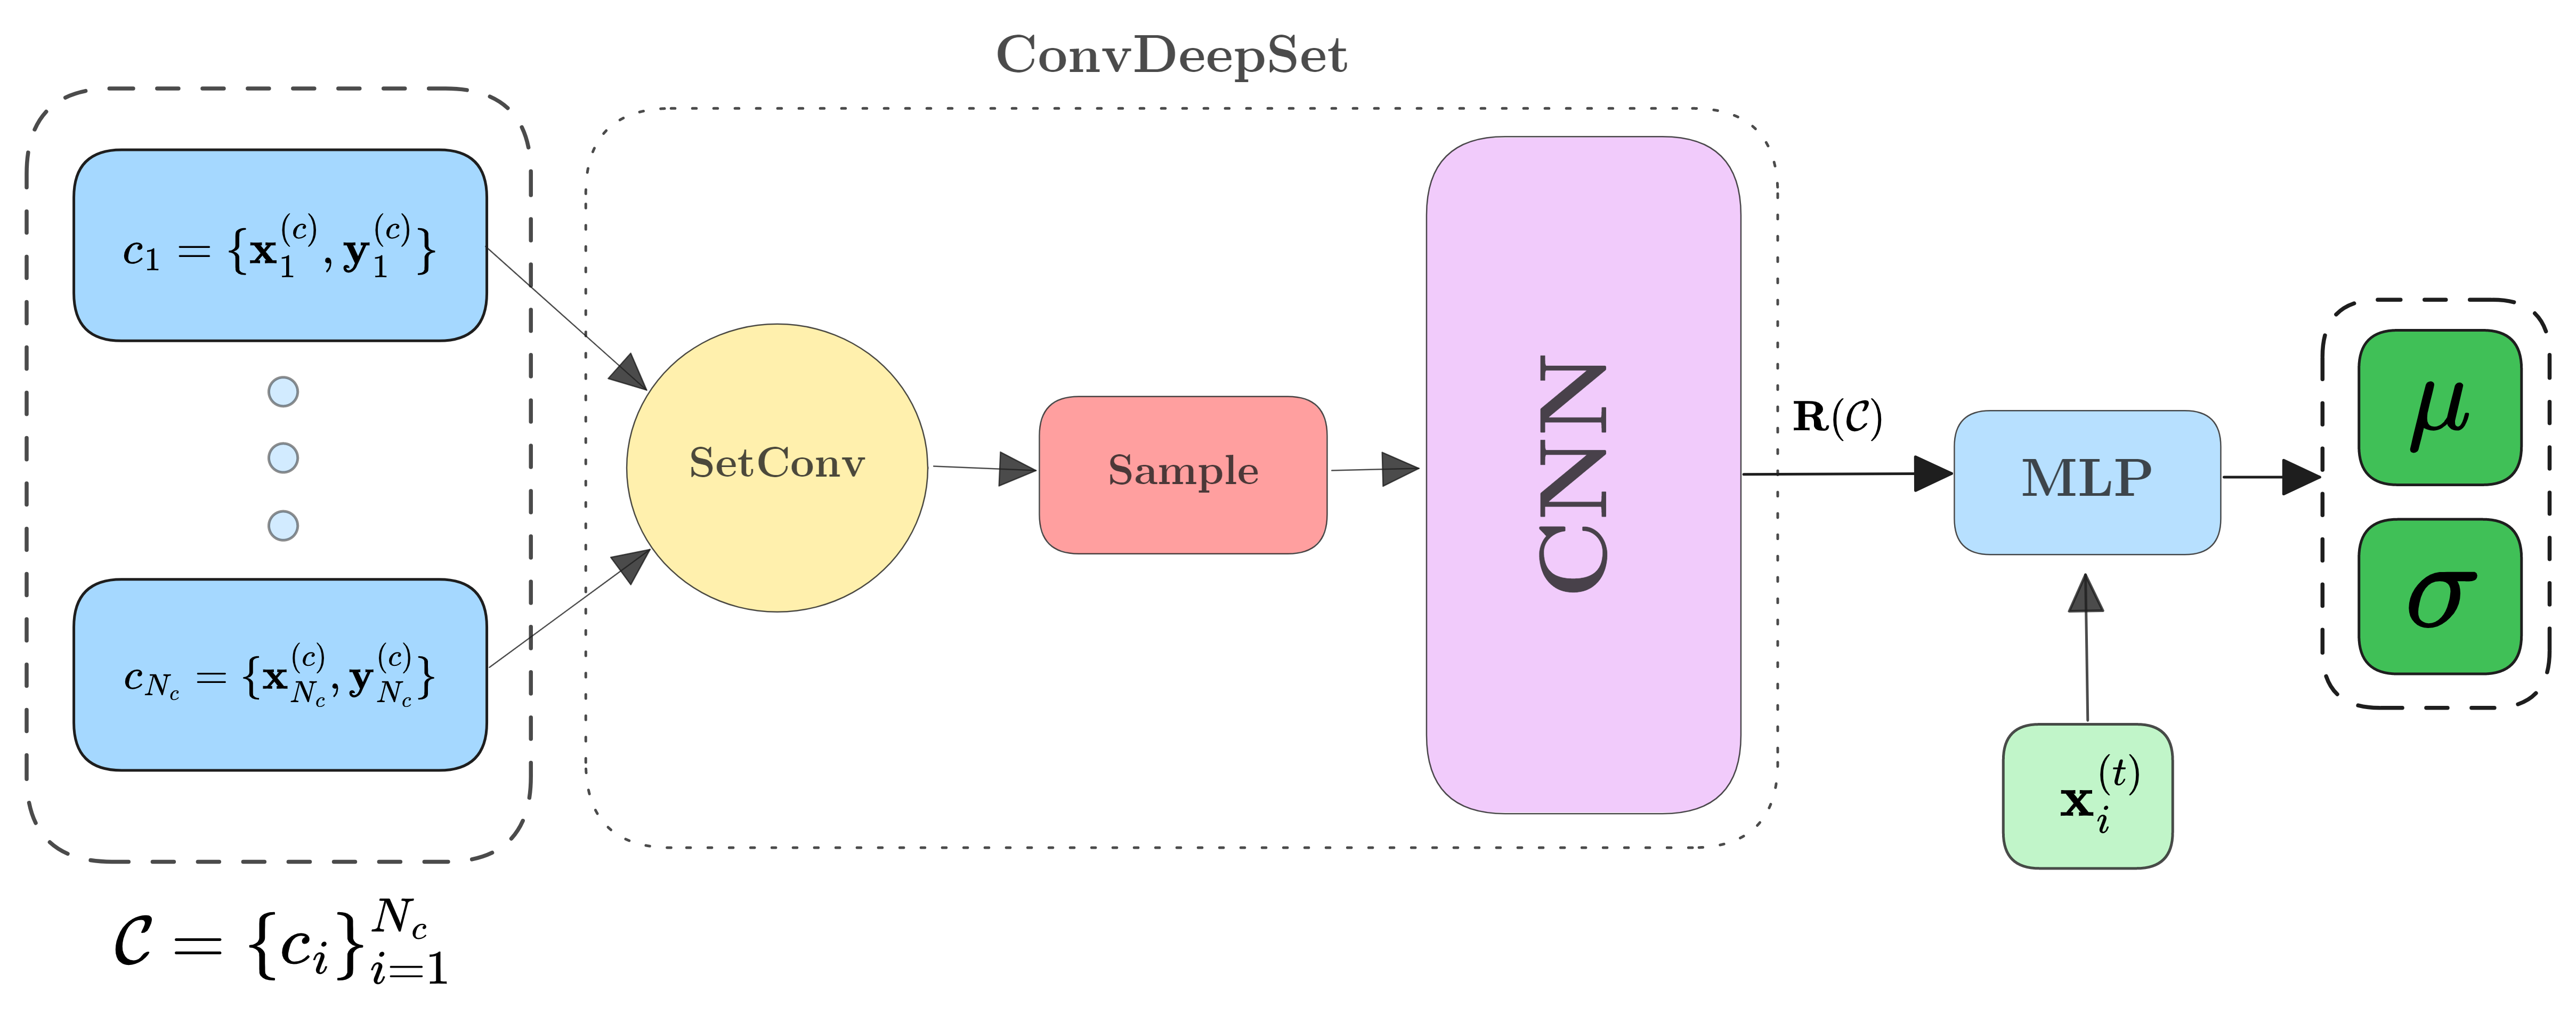
\includegraphics[width=0.8\textwidth]{convcnp.png}
	\caption{ConvNP Architecture. All the data points are transformed into a continuous functional embedding using the SetConv, then discretely sampled to be fed into a CNN. The CNN processes the data whose output is converted back to a continuous function using the SetConv operation.}
	\label{fig:convcnp}
\end{figure}


CNNs operate on \textbf{on-grid data}, implying the data is on a regular grid, such as an image. However, the data we are working with is sometimes \textbf{off-grid data}, e.g. time series dataset with irregular timestamps. Furthermore, to `bake-in' the translation equivariance property, we need to be able to shift the data in the input space and the output space consistently. This is not trivial when using standard vector representations of the data as there is no inherent notion of translation in a vector.
\cite{gordon2020convolutional} propose a solution to this problem by using \textbf{functional embeddings} to model the discrete data as \emph{continuous functions}. With functional embeddings, the data can be translated in the input space and the output space consistently thus permitting translation equivariance.

The \textbf{SetConv} operation takes a set of input-output pairs and outputs a continuous functional representation of the data as follows:

\begin{equation}
	\label{eq:setconv}
	\text{SetConv}(\{\bm{x_i}, \bm{y_i}\}_{i=1}^{N})(x) = \sum_{i=1}^{N} [1, \bm{y_i}] ^ T \mathcal{K}(\bm{x} - \bm{x_i})
\end{equation}

Where $\mathcal{K}$ is a kernel function that measures the distance between the query $x$ and the data point $\bm{x_i}$.

This operation has some key properties:
\bul{
	\item We append $1$ to output $\bm{y_i}$ when computing the SetConv, this acts as a flag allowing the  model to knows which data points are observed and which are not. Say we have a data point of $\bm{y_i} = 0$, then if we did not append the $1$, the model would not be able to distinguish between an observed data point and an unobserved data point (as both would be $0$).
	\item The `weight' of the kernel depends only on the \emph{relative distance} between points on the input space hence the model is translation equivariant.
	\item The summation over the data points naturally introduces \textbf{Permutation Invariance} to the model.
}


The function representation of the context set, is sampled at \textbf{evenly} spaced points giving us discrete data in a \textbf{on-grid} format. It is then fed into a CNN. After the CNN processes the data, it need to convert it back to a continuous function by using the SetConv operation. The final output of the encoder is a continuous function that represents the context set which can be queried at any point in the input space using the target set, given by:

\begin{equation}
	R(\bm{x_t}) = \text{SetConv}(\text{CNN}(\{\text{SetConv}(\mathcal{C})(\bm{x_d})\}_{d=1}^{D}))(\bm{x_t})
\end{equation}

The decoder is a simple MLP that takes the output of the encoder and the target set as input and generates the mean and variance of the predictive distribution $\bm{\mu}(\bm{x_t}), \bm{\sigma}(\bm{x_t}) = \text{MLP}(R(\bm{x_t}))$


\ifSubfilesClassLoaded{%
    \printbibliography{}
}{} 


\end{document}